\documentclass[10pt,a4paper]{article}
\usepackage[margin=18mm]{geometry}
\usepackage[T1]{fontenc}
\usepackage{lmodern,graphicx,booktabs,amsmath,amssymb}
\usepackage[hidelinks]{hyperref}
\setlength{\parindent}{0pt}
\setlength{\parskip}{5pt}
\begin{document}
{\Large\bfseries Actual mixed Jacobian chain over the prime field}\par
23 November 2026 \quad Native correctness and written geometry [pcc:unverified]

\textbf{Outcome.} The fixed mixed map is a genuine degree-64 endomorphism
of $J=\operatorname{Jac}(C_7)$ over $\mathbb F_7$. Its complete kernel has
type $(4,4,2,2)$ and is Frobenius stable and maximally isotropic. Its
integral Rosati adjoint composes with it in both orders to $[4]$.
The complete native torsion and rational-point certificates verify the
fixed finite cohorts. Data8b15b2; standard geometric dependencies remain
explicit in the source proof.

\begin{center}
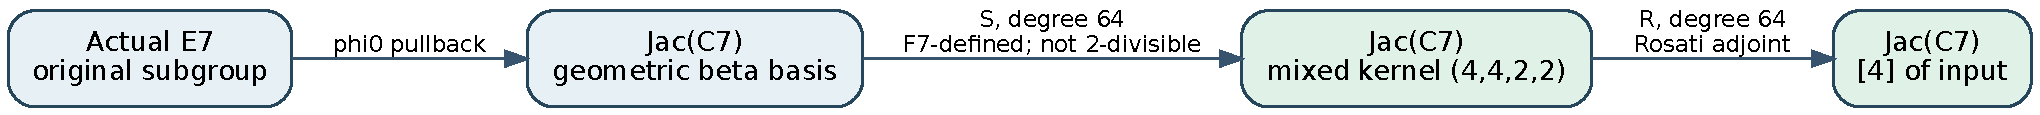
\includegraphics[width=\linewidth,height=44mm,keepaspectratio]{chain.pdf}
\end{center}

\textbf{The actual bridge.} For the genuine degree-two/two/three covers,
$g=(\phi_0-\phi_1-\phi_3\pi)/3$ descends through the certified geometric
$E_7[3]$ kernel. The actual isomorphism
$\beta=(\phi_1,-g,g-\phi_3):E_7^3\to J$ has Gram $H$ with determinant
one. Put $\alpha=\beta^{-1}$, $\omega=\pi+2$,
$\omega^2-\omega+5=0$. Transport the fixed matrices by $\beta$:
\[
S=\begin{pmatrix}-4&-2&2\\2+2\omega&-1+2\omega&-1-2\omega\\
-4+2\omega&-3+\omega&3-\omega\end{pmatrix},\quad
R=\begin{pmatrix}-3+\omega&0&2\\4&-2&-2\omega\\
2\omega&-2&4-2\omega\end{pmatrix}.
\]
$S^\dagger HS=R^\dagger HR=4H$ and $RS=SR=4I$. Hence the genuine maps
$S_J=\beta S\alpha$, $R_J=\beta R\alpha$ have degree64 and compose to
$[4]$. The geometric bridge legitimizes these coordinates; no synthetic
Jacobian or native genus-three reduction engine is substituted.

\begin{center}
\begin{tabular}{lrp{79mm}}
\toprule
Fixed cohort & Complete count & Observed qualification\\
\midrule
Division-factor scan &117649& Six roots; every accept/reject bit retained\\
Actual $E_7[4]$ &16& Full group/Frobenius; actual Weil basis indices4,6\\
Actual Weil4 pairings &256& $T$ and $2T$ agree; primitive $i=3b$;216 changed-line rejections\\
Whole C7 fibre schemes &15& Curve, forward-target, origin-jet and $R$ identities\\
Actual $J[4]$ decisions &4096& Full $S/R$/Frobenius maps through $\beta$\\
Full kernel pairings &4096& All are1;64-point kernel,16 killed by2,48 of order4\\
Rational $J(\mathbb F_7)$ &1331& $S/R$ bijections, both composites$[4]$\\
Original elliptic scalars &11& Preserved/recovered;10 changed-map rejections\\
\bottomrule
\end{tabular}
\end{center}

$S(J[2])$ has four elements, proving genuine nondivisibility by$[2]$.
On all64 actual $J[2]$ points, $\pi^2+\pi+I=0$. The irreducible
$\mathbb F_4$-module structure forces every Frobenius-stable subspace
to have even $\mathbb F_2$ dimension; there is no dimension-three
$\mathbb F_7$ Lagrangian for a $(2,2,2)$ first step. This written
consequence leaves extension-field factorizations open.
\newpage
{\Large\bfseries Global split transfer and a primitive degree-four cover}\par
\textbf{Written extension after the native run.} The original elliptic
embedding has $\beta$ column $v=(1,-1-\omega,2-\omega)^t$. Exact
coefficient multiplication gives
\[
 u=Sv=(2,1-2\omega,5-\omega)^t,\quad
 \ell=(\omega,1,0),\quad \ell u=1.
\]
Thus $\tau=S_J\phi_0=\beta u$ has the genuine integral global left
inverse $L=\ell\alpha$. This preserves a discrete-log scalar on every
subgroup. It is a written Hom identity, not a new nativeB branch.
The fixed inverse $H$ gives
\[
 \ell H^{-1}=(\omega-1,-\omega,-2),\qquad
 LL^\dagger=\ell H^{-1}\ell^\dagger=4.
\]
The curve map $f_4(P)=L([P-P_-])$ therefore has degree4 by standard
Jacobian push-pull. Its rational functions remain uncomputed.

\textbf{Prime-field factorization obstruction.} The earlier complete
canonical-frame census gives $\operatorname{Aut}_{\mathbb F_7}(C_7)=S_3$;
all three involutions have genus-one quotients. A degree-two-by-two
factorization of $f_4$ over $\mathbb F_7$ would therefore have an elliptic
middle curve and a degree-two elliptic isogeny into $E_7$. Its dual
would require a rational order-two point on $E_7$, contradicting
$\#E_7(\mathbb F_7)=11$. The cover is primitive over the prime field.
No claim about geometric monodromy or extension-field factors is made.

\textbf{Finite-point guard.} The exact pushforward formula is
\[
 3L=\pi f_{0*}+(2\pi+3)f_{1*}-f_{3*}.
\]
On rational order11 points one may multiply its numerator by4 to get
$L$. Globally that substitution is $[12]L$, yielding a degree576 curve
map which agrees with $f_4$ on all rational points. Finite-point
interpolation cannot establish the desired degree-four rational
functions; genuine function-field division and degree/chart checks
are still required.

\textbf{Concrete rational transfer.} For $T=(1,3)$, nativeB gives
$\phi_0(T)=(1,7,10)T$ and $S_J\phi_0(T)=(2,6,2)T$ in actual
$\beta$ coordinates. The image leaves the original elliptic subgroup.
All11 scalar targets recover through $R_J$ and inverse4 modulo11.
The global left inverse above is stronger than this bounded recovery.

\textbf{Execution and originals.} Frozen sourceB\texttt{257bf0f}
had all69 full input/lock readbacks before first B calls. All seven
strict phases exit zero, guards unchanged: Rust1.99.1, warnings denied,
overflow/debug assertions, one worker,120seconds/2GiB per phase.
FirstA passed format/compile then failed Clippy on parity style before
science; all31 originals and597-byte diagnostic remain. B changes only
the parity method and CM module path, preserving all26 frozenA inputs.

The original complete13-section certificate is59325bytes,
SHA256\texttt{2fb5d882\ldots{}3189b37}; full stdout28981bytes,
\texttt{56cb216e\ldots{}5dbbb23}. All39 small originals were published
and read back in full at\texttt{62db83d}. The original whole4762952-byte
executed ELF\texttt{3ec7fe57\ldots{}60d25c8e} remains in RAM pending
approved durable custody. No scientific rerun or policy/limit change.

\textbf{Continuation.} Next independently verify the complete packet
with a different field presentation and a third Miller auxiliary;
then derive explicit degree-four functions and genuine divisor/target
evaluation. Generic Lean, signed external review and quantitative
cold-cost admission remain separate. All maps are $\mathbb F_7$-defined;
the degree-six field computes geometric torsion and is not a proper
subfield DLP descent. Required CI/ledger blockers stay recorded.

\href{https://github.com/isogeny-labs/crypto/tree/257bf0f170d578d268454813a093de270c9906c5/research/chained_cm19_actual_j4_20261123}{Frozen source and firstA negative}.\par
\href{https://github.com/isogeny-labs/crypto/tree/62db83d43c31b028fa8fb68be94bf2caa2b53845/research/chained_cm19_actual_j4_20261123}{Complete certificate and written proofs}.\par
Data8b15b2, written3c0acb/d431a8; finite-point guard38ae70.
KB/Conductor unavailable; no novelty clearance. [pcc:unverified]
\end{document}
